% ============================================================================
%  paper.tex
%
%  Semantic Reduction Is the Bottleneck:
%  A Three-Layer Reliability Framework for AI for Mathematics
%
%  Compile with:  pdflatex paper && bibtex paper && pdflatex paper && pdflatex paper
%  (also compiles under xelatex)
%
%  Self-contained: uses only packages from a standard TeX distribution.
% ============================================================================
\documentclass[11pt,a4paper]{article}

% ---------- encoding & fonts ----------
\usepackage[utf8]{inputenc}
\usepackage[T1]{fontenc}
\usepackage{lmodern}

% ---------- layout ----------
\usepackage[margin=1in]{geometry}
\usepackage{microtype}

% ---------- math ----------
\usepackage{amsmath,amssymb,amsthm}
\usepackage{mathtools}

% ---------- graphics & tables ----------
\usepackage{graphicx}
\usepackage{booktabs}
\usepackage{array}
\usepackage{tabularx}
\usepackage{multirow}
\usepackage{xcolor}

% ---------- algorithms ----------
\usepackage{algorithm}
\usepackage{algpseudocode}

% ---------- code listings ----------
\usepackage{listings}

% ---------- captions, urls, references ----------
\usepackage[font=small,labelfont=bf]{caption}
\usepackage[hidelinks]{hyperref}
\usepackage{url}

% ---------- theorem environments ----------
\theoremstyle{definition}
\newtheorem{definition}{Definition}[section]
\theoremstyle{plain}
\newtheorem{proposition}{Proposition}[section]
\newtheorem{lemma}[proposition]{Lemma}
\theoremstyle{remark}
\newtheorem{remark}{Remark}[section]
\newtheorem{example}{Example}[section]

% ---------- listings style ----------
\definecolor{codegray}{gray}{0.95}
\definecolor{codecomment}{rgb}{0.35,0.45,0.55}
\definecolor{codekw}{rgb}{0.10,0.30,0.60}
\lstdefinestyle{plain}{
  basicstyle=\ttfamily\footnotesize,
  backgroundcolor=\color{codegray},
  commentstyle=\color{codecomment}\itshape,
  keywordstyle=\color{codekw}\bfseries,
  breaklines=true,
  frame=single,
  rulecolor=\color{gray!40},
  showstringspaces=false,
  columns=fullflexible,
  xleftmargin=6pt,
  xrightmargin=4pt,
  aboveskip=8pt,
  belowskip=8pt
}
\lstset{style=plain}

% ---------- convenience macros ----------
\newcommand{\NL}{\mathcal{N}}          % natural language space
\newcommand{\IR}{\mathcal{I}}          % IR space
\newcommand{\FS}{\mathcal{F}}          % formal system
\newcommand{\red}{\rho}                % semantic reduction map
\newcommand{\Anch}{\mathsf{Anchor}}
\newcommand{\V}{\mathcal{V}}           % verifiability score
\newcommand{\sem}[1]{\llbracket #1 \rrbracket}

\title{\bfseries Semantic Reduction Is the Bottleneck:\\ A Three-Layer Reliability Framework for AI for Mathematics}

\author{%
  \textit{Elite~20 Program} \\[2pt]
  \small AI4Math Reliability Study Group
}

\date{September 2026}

\begin{document}
\maketitle

% ============================================================================
\begin{abstract}
\noindent
Large language models can now produce mathematical proofs that read as expert
work, and they can also produce proofs that are subtly and irreparably wrong.
The reliability question for AI for Mathematics (AI4Math) is therefore not
``can the model solve the problem?'' but ``when the model says it has solved
the problem, how much should we believe it?'' Current answers fall into two
families: \emph{post-hoc verification}, which checks a finished natural-language
proof with an external tool, and \emph{end-to-end formalisation}, which asks the
model to emit a proof directly in a proof assistant such as Lean.
We argue that both families mislocate the difficulty, and we place the failure
mode in a specific architectural position.

We propose a three-layer decomposition of AI4Math systems---\emph{generation},
\emph{semantic reduction}, and \emph{verification}---and argue that the
semantic reduction layer, which maps informal mathematical claims onto typed
formal objects, is the dominant bottleneck. We formalise this claim by
introducing a typed intermediate representation (SRIR) with an explicit
anchoring map, defining a \emph{verifiability score} $\V(x)$ that separates
anchored from unanchored fragments of a derivation, and giving a taxonomy of
seven reduction defects. We then present a falsifiable prediction: the
\emph{narrowing hypothesis}, that a system's error rate at fixed solution effort
is bounded by its unanchored fraction. Finally we give a reusable
\emph{Reliability Checklist} for auditing AI4Math claims, and we state the
boundary conditions under which our analysis does and does not apply.

The contribution is conceptual and methodological rather than empirical: we do
not report large-scale experiments, and we are explicit that the framework is
motivated by, and consistent with, published results rather than proved by
them. Our aim is to give researchers and practitioners a vocabulary precise
enough to locate reliability failures, and a checklist precise enough to act on
them.
\end{abstract}

\noindent\textbf{Keywords:} AI for Mathematics, autoformalisation, proof
assistants, neuro-symbolic reasoning, reliability, verifiability, hallucination.

% ============================================================================
\section{Introduction}
\label{sec:intro}

\subsection{The reliability gap}

Between 2022 and 2026, machine mathematical reasoning moved from word problems
to research-adjacent results. Systems trained with reinforcement learning
against a proof assistant reached medal-level performance on olympiad problems
\cite{hubert2026olympiad,chervonyi2025gold}; the same neuro-symbolic recipe
rediscovered algorithms that had resisted human search for decades
\cite{fawzi2022discovering,romera2024mathematical}; and language models
fine-tuned on mathematical corpora began to produce fluent, confident,
multi-step arguments \cite{azerbayev2024llemma}.

Fluency, however, is not correctness. A model that has learned the
\emph{register} of mathematical prose has learned to produce text that looks
like a proof, and the surface features that distinguish a valid proof from an
invalid one---whether a limit interchange is licensed, whether an induction is
well-founded, whether a cited lemma's hypotheses are actually met---are exactly
the features that a next-token predictor has no direct incentive to preserve.
Empirical work has repeatedly found that apparent mathematical competence
degrades sharply once the task requires genuine multi-step composition rather
than pattern retrieval \cite{frieder2023mathematical}. The gap between
``produces a proof-looking object'' and ``produces a proof'' is the reliability
gap.

\subsection{Two answers, and why they are incomplete}

The field's response has been to add a verifier.

\emph{Post-hoc verification} takes the model's natural-language proof and
subjects it to an external check: a symbolic engine, an SMT solver, or a
critic model. This is attractive because it is cheap and does not constrain the
generator. It is also structurally weak: if the natural-language derivation
contains an unstated inference, a symbol the checker cannot type, or an
implicit appeal to ``standard facts,'' then the checker either fails on a
correct proof or---worse---succeeds on an incorrect one by checking a weaker
formalisation than the author intended.

\emph{End-to-end formalisation} bypasses this by asking the model to emit a
proof directly in a proof assistant. When it succeeds, the resulting artifact
is checkable by a small trusted kernel and its correctness is as certain as the
foundations allow \cite{demoura2015lean,mathlib2020lean}. This is the strongest
available notion of reliability, and it is why the strongest systems use it.
But it does not remove the difficulty; it relocates it. The model must now
produce a \emph{formal} object, and the mapping from the informal statement a
human asked about to the formal statement the kernel checks is performed by the
model itself, in natural language, before any verification happens. If that
mapping is wrong, the kernel will faithfully certify a theorem nobody asked
about.

\subsection{Thesis}

We argue that both answers share a blind spot: they treat the transition from
informal mathematics to formal mathematics as an implementation detail. We claim
it is the central object of study. Concretely:

\begin{quote}
\textbf{Thesis.} In a layered AI4Math system, the dominant source of
reliability failure is neither the generator nor the checker, but the
\emph{semantic reduction layer} that maps informal mathematical content onto
typed formal objects. Reliability therefore cannot be obtained by improving
the final check alone; it requires making the reduction layer an explicit,
instrumented, and auditable system component.
\end{quote}

This is a claim about where difficulty lives, and it is falsifiable in the
sense that a system could be exhibited whose reduction is demonstrably faithful
and whose residual errors lie elsewhere. We state the conditions under which we
expect the thesis to fail in Section~\ref{sec:boundary}.

\subsection{Contributions}

\begin{enumerate}
  \item \textbf{A three-layer decomposition} of AI4Math systems
        (Section~\ref{sec:layers}) that separates generation, semantic
        reduction, and verification, and that makes the interfaces between them
        explicit and \emph{instrumentable}.

  \item \textbf{A typed intermediate representation (SRIR)} with a formal
        anchoring map $\Anch$ and a notion of \emph{semantic closure}
        (Section~\ref{sec:srir}), designed so that every node of a derivation is
        either anchored to a checkable object or explicitly marked as
        unanchored.

  \item \textbf{A verifiability measure $\V(x)$} (Section~\ref{sec:verifiability})
        that quantifies the anchored fraction of a derivation, together with a
        taxonomy of seven reduction defects
        (Section~\ref{sec:taxonomy}) that gives failures names.

  \item \textbf{The narrowing hypothesis} (Section~\ref{sec:hypothesis}): a
        falsifiable, testable statement connecting the unanchored fraction of a
        derivation to residual error rate, with a proposed experimental design
        and explicit confounders.

  \item \textbf{A Reliability Checklist} (Section~\ref{sec:checklist} and
        Appendix~\ref{app:checklist}) for auditing AI4Math claims in practice.
\end{enumerate}

\subsection{Scope and non-claims}

This paper is a position and framework paper. We do not report new experiments,
we do not claim superiority over existing systems, and we do not claim that the
semantic reduction layer is the \emph{only} source of unreliability. Sections
\ref{sec:boundary} and \ref{sec:discussion} state the limits of the analysis
explicitly. Where we cite empirical numbers, they are from the cited primary
sources and are used to motivate the framework, not to validate it.

% ============================================================================
\section{Background and Related Work}
\label{sec:related}

\subsection{Proof assistants and the trusted kernel}

Interactive theorem provers (ITPs) such as Coq, Isabelle, and Lean rest on a
small trusted kernel that checks each inference against a fixed set of rules
\cite{maric2015survey}. The Lean prover and its mathematical library,
\texttt{mathlib}, provide a modern instantiation with a large, machine-readable
body of formalised mathematics \cite{demoura2015lean,mathlib2020lean}. The
architectural property that matters for us is the \emph{de Bruijn criterion}:
all proof construction, however clever or however unreliable, is reduced to a
check against a small kernel. This makes the kernel an \emph{absolute} oracle
for the formal claim it is given---and a silent bystander to the question of
whether that formal claim is the intended one.

That gap---between the intended claim and the formalised claim---is the space
our framework is designed to make visible. We call it the \emph{anchoring
gap}.

\subsection{Autoformalisation}

Autoformalisation is the task of translating informal mathematical statements
and proofs into formal ones. Wu et al.\ \cite{wu2022autoformalization}
established that large language models can perform this translation with useful
but imperfect accuracy, reporting that a substantial fraction of translated
statements are syntactically well-formed yet semantically divergent from their
sources. Zhou et al.\ \cite{zhou2024donttrust} turn this into a reliability
mechanism: formalise the model's own reasoning and let the checker veto it,
finding that verification-by-autoformalisation outperforms majority voting on
grade-school arithmetic.

This line is the closest to our position, and our contribution is
complementary rather than competing. Prior work treats autoformalisation as a
\emph{step} whose output may be filtered. We treat it as a \emph{layer} whose
internal structure determines the ceiling on achievable reliability, and we
provide a representation and a metric that make the layer's residual
unreliability measurable rather than merely detectable in aggregate.

\subsection{Neural--symbolic theorem proving}

The strongest current systems pair a learned policy with a proof assistant.
AlphaProof formalises olympiad problems, searches with a learned value function
and tree search, and certifies every successful proof in Lean; it reached
silver-medal level at IMO 2024 \cite{hubert2026olympiad}. AlphaGeometry2
similarly attains gold-medal-level geometry performance using a dedicated
domain representation and a symbolic deduction engine \cite{chervonyi2025gold}.
Open systems such as Goedel-Prover and retrieval-augmented provers such as
LeanDojo push these capabilities into reproducible, open-weight territory
\cite{lin2025goedel,yang2023leandojo}. Yang et al.\ survey the resulting
research programme \cite{yang2024formal}.

These systems demonstrate that the neuro-symbolic loop works. They also
illustrate our thesis in their own deployment reports: capability is bounded by
the coverage of the formal library and by the fidelity of the informal-to-formal
translation, not by the search procedure. Geometry required a separate system
precisely because the shared formal library did not cover olympiad-style
geometry well enough to make reduction reliable
\cite{chervonyi2025gold}. That is a reduction-layer failure dictating an
architectural workaround.

\subsection{Language models for mathematics and step-level verification}

Llemma demonstrates that continued pretraining on mathematical and code corpora
yields a substantially stronger informal reasoner
\cite{azerbayev2024llemma}. Chain-of-thought prompting elicits multi-step
derivations by making intermediate steps explicit
\cite{wei2022chain}. Step-level supervision goes further, rewarding correct
\emph{process} rather than only correct outcomes, and producing models that can
localise their own errors
\cite{lightman2023verify}. The relevance to us is direct: step-level
verification presupposes that steps are \emph{identifiable objects} with
checkable content, which is exactly what the SRIR representation of
Section~\ref{sec:srir} provides, and exactly what raw natural-language
derivations lack.

\subsection{Benchmarks and what they measure}

GSM8K and MATH measure final-answer correctness on word problems and
competition mathematics respectively \cite{cobbe2021training,hendrycks2021measuring}.
DeepMath-Creative measures creativity along three axes---new concepts, new
methods, and new examples---and finds that current models struggle most on
tasks requiring genuine construction \cite{chen2025deepmath}. Frieder et al.\
document sharp degradation of apparent mathematical competence under careful
evaluation \cite{frieder2023mathematical}.

The methodological point we take from this literature is that
\emph{answer-level} benchmarks cannot distinguish a model that reasoned
correctly from one that arrived at a correct answer through invalid steps. Our
$\V(x)$ measure is an attempt to supply the missing axis: not whether the
answer is right, but how much of the derivation is anchored.

\subsection{What is missing}

Across this literature the reduction step is variously treated as a
preprocessing detail, a filtering mechanism, or an implicit competence. We are
not aware of a framework that (i)~gives informal-to-formal reduction its own
architectural layer with defined interfaces, (ii)~assigns each derivation node
an explicit anchoring status, and (iii)~yields a scalar measure that can be
tracked across systems. Providing these is the contribution of this paper.

% ============================================================================
\section{A Three-Layer Decomposition}
\label{sec:layers}

\subsection{The layers}

We decompose any AI4Math system that aspires to verifiable output into three
layers with typed interfaces.

\begin{definition}[Three-layer decomposition]
\label{def:layers}
An AI4Math system is a tuple $\langle G, R, C \rangle$ where:
\begin{itemize}
  \item $G:\NL \to \NL$ is the \textbf{generation layer}, mapping an informal
        problem statement to an informal derivation;
  \item $R:\NL \to \IR$ is the \textbf{semantic reduction layer}, mapping
        informal mathematics to typed formal objects in an intermediate
        representation $\IR$ (Section~\ref{sec:srir});
  \item $C:\IR \to \{\top,\bot\}$ is the \textbf{verification layer},
        deciding whether a formal object is accepted by the target formal
        system $\FS$.
\end{itemize}
The system's output on input $p$ is $C(R(G(p)))$.
\end{definition}

The composition in Definition~\ref{def:layers} is deliberately simple; its
point is to expose that a single user-visible verdict is the product of three
independently unreliable components.

\subsection{Why the middle layer is where failures concentrate}

Each layer has a characteristic failure mode.

\paragraph{Layer 1 (generation) fails by producing wrong content.}
This failure is \emph{loud}: the derivation is wrong, and any downstream check
that has enough information can catch it. Crucially, $G$ operates in $\NL$,
where the notion of ``wrong'' is itself contested.

\paragraph{Layer 3 (verification) fails by being incomplete.} A kernel may
reject a valid proof (incompleteness, resource limits) but, by the de Bruijn
criterion, it does not accept invalid proofs. Its failure mode is conservative
and detectable: rejection.

\paragraph{Layer 2 (semantic reduction) fails by being \emph{silently
unfaithful}.} The reduction may map an informal claim to a formal claim that is
checkable, syntactically well-formed, \emph{and not the claim the user meant}.
Every downstream component then behaves correctly with respect to the wrong
target. This is the only failure mode in the system that is simultaneously
(i)~undetectable by the verifier, (ii)~indistinguishable from success at the
user interface, and (iii)~able to corrupt a proof that is internally flawless.

\begin{proposition}[Asymmetry of detectability]
\label{prop:asymmetry}
Let $C$ satisfy the de Bruijn criterion. Then:
\begin{enumerate}
  \item Every error introduced at Layer~3 is either detectable as a rejection
        or absent.
  \item Errors introduced at Layer~2 are not detectable by $C$ alone whenever
        the reduced object is internally consistent.
\end{enumerate}
\end{proposition}

\begin{proof}[Proof sketch]
(1) holds by definition of the de Bruijn criterion: $C$ accepts only objects
derivable in $\FS$, so an invalid object yields $\bot$. (2) Suppose $R$ maps
claim $\varphi$ to formal object $i \neq R(\varphi)$ but $i$ is derivable in
$\FS$; then $C(i) = \top$ while the intended claim is unverified. No property of
$C$ alone can distinguish this case from a faithful reduction, since $C$ has
access only to $i$ and not to $\varphi$.\qed
\end{proof}

Proposition~\ref{prop:asymmetry} is the formal core of our thesis. Note what it
does \emph{not} say: it does not claim Layer~2 errors are the most frequent, nor
that Layers~1 and~3 are unimportant. It claims that Layer~2 errors are uniquely
invisible to the verification layer, and therefore cannot be addressed by
strengthening verification. This is a statement about \emph{where additional
verification effort has no leverage}, which is precisely the kind of statement
that should guide architecture.

\begin{figure}[t]
\centering
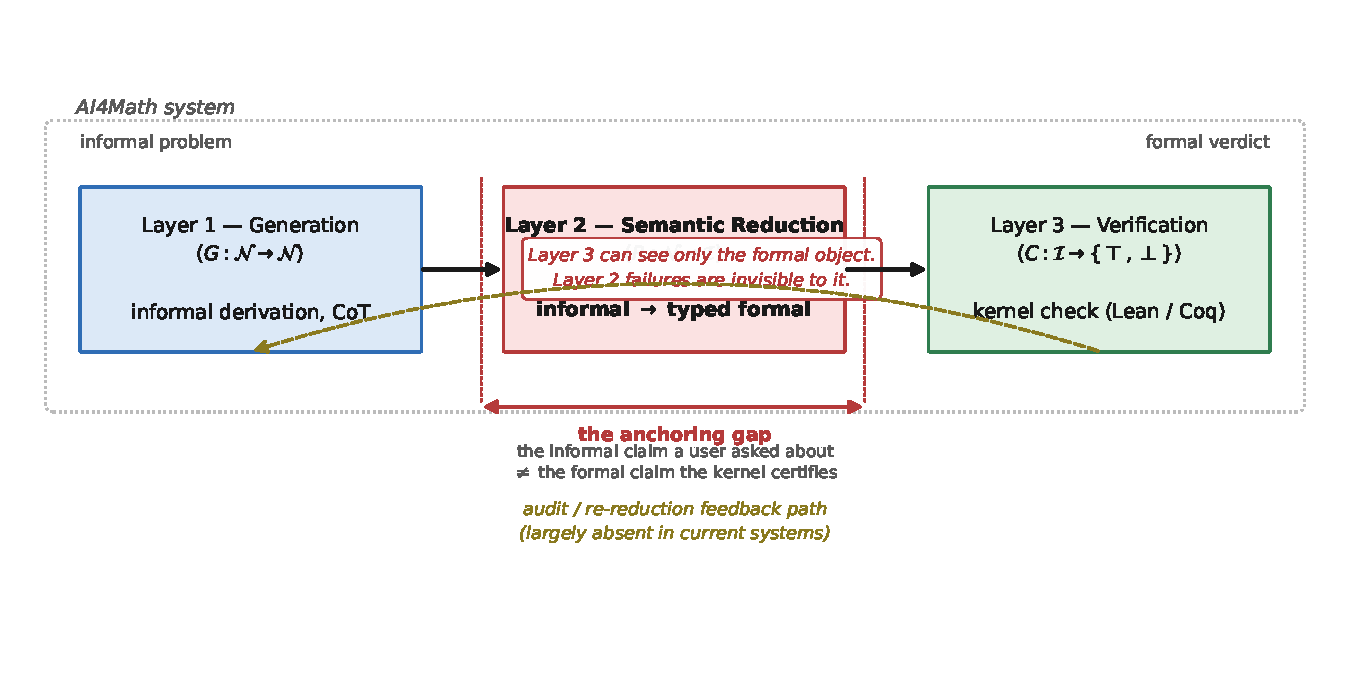
\includegraphics[width=0.86\textwidth]{fig1_architecture.pdf}
\caption{The three-layer decomposition. Solid arrows are the data path;
the dashed arrow is the feedback path that current systems largely omit. The
\emph{anchoring gap} is the distance between the informal claim a user asked
about and the formal claim the kernel certifies. Layer~2 is the only layer whose
failures are invisible to Layer~3 (Proposition~\ref{prop:asymmetry}).}
\label{fig:arch}
\end{figure}

\subsection{The pipeline as a contract}

Read left to right, Figure~\ref{fig:arch} describes a pipeline. Read as a
contract, it imposes obligations. Layer~1 owes Layer~2 a derivation whose steps
are \emph{individually identifiable}. Layer~2 owes Layer~3 formal objects that
are \emph{type-correct and semantically anchored}. Layer~3 owes the system a
verdict on \emph{exactly the object it was given}. Most current systems satisfy
the third obligation rigorously and the first two informally---which is
consistent with the empirical pattern that verification is reliable and
reliability overall is not.

% ============================================================================
\section{SRIR: A Typed Intermediate Representation}
\label{sec:srir}

\subsection{Design goals}

We want a representation that makes the anchoring gap \emph{measurable}. Four
requirements follow directly from the failure analysis above.

\begin{enumerate}
  \item \textbf{Step identity.} Every inference step must be a first-class
        object with a stable identifier, so that anchoring can be assessed
        per step rather than per proof.
  \item \textbf{Explicit typing.} Every object must carry a type, so that
        type mismatch---a common silent failure---becomes a checkable
        condition rather than a plausibility judgement.
  \item \textbf{Explicit dependencies.} Each step must declare which prior
        steps and which library facts it consumes, so that an unanchored
        dependency cannot hide behind a fluent sentence.
  \item \textbf{Explicit unanchored status.} A step that cannot be anchored must
        be \emph{representable as unanchored}. The representation must not force
        a choice between ``anchored'' and ``absent.''
\end{enumerate}

Requirement~4 is the one that distinguishes SRIR from a proof object. A proof
object records what was proved; SRIR records what was \emph{claimed} and how
much of it was \emph{secured}.

\subsection{Definition}

\begin{definition}[SRIR graph]
\label{def:srir}
An SRIR document is a finite directed acyclic graph
$\mathcal{G} = (V, E, \tau, \delta, \alpha)$ where:
\begin{itemize}
  \item $V$ is a finite set of \emph{derivation nodes}, the steps;
  \item $E \subseteq V \times V$ encodes dependency: $(u,v) \in E$ means $v$
        consumes the result of $u$;
  \item $\tau : V \to \mathcal{T}$ assigns each node a type drawn from a type
        system $\mathcal{T}$ that includes at least \textsf{Prop},
        \textsf{Term}, \textsf{Assumption}, \textsf{LemmaRef}, and
        \textsf{Goal};
  \item $\delta : V \to \FS$ assigns each node a formal counterpart in the
        target system $\FS$ (a term, a proof obligation, or a goal state);
  \item $\alpha : V \to \{\mathsf{A}, \mathsf{U}\}$ is the \emph{anchoring
        status}: $\alpha(v) = \mathsf{A}$ (\emph{anchored}) iff $\delta(v)$ is
        well-typed, references only library facts that exist in $\FS$, and is
        accepted by the kernel when its dependencies are discharged;
        $\alpha(v) = \mathsf{U}$ (\emph{unanchored}) otherwise.
\end{itemize}
\end{definition}

The \emph{anchored subgraph} $\mathcal{G}_A = (V_A, E_A)$ is the restriction of
$\mathcal{G}$ to $V_A = \{v : \alpha(v) = \mathsf{A}\}$.

\begin{definition}[Semantic closure]
\label{def:closure}
$\mathcal{G}$ is \emph{semantically closed} if $\alpha(v) = \mathsf{A}$ for the
root node and every node in the transitive dependency cone of the root.
\end{definition}

Semantic closure is the property a system should aim for: not merely that the
final answer is certified, but that the certification does not rest on any
unanchored step.

\subsection{The anchoring map and the anchoring gap}

\begin{definition}[Anchoring map]
\label{def:anchormap}
The anchoring map $\Anch : \NL \to \IR$ is the concrete realisation of the
semantic reduction layer $R$: it sends an informal mathematical claim to an
SRIR node whose formal counterpart is $\delta(v)$. The \emph{anchoring gap} of
a reduction is the pair $(\varphi, \delta(\Anch(\varphi)))$---the informal claim
and the formal object that will actually be checked in its place.
\end{definition}

The anchoring gap is not a defect. It is unavoidable: informal mathematics runs
on shared understanding, and any formalisation must choose a specific rendering.
The question that matters is whether the gap is \emph{disclosed}. A system that
emits a Lean file and a natural-language gloss, with no correspondence between
them, has an undisclosed gap; a system that emits an SRIR graph in which every
node carries its informal gloss, its type, and its anchoring status has a
disclosed one. Disclosure is what makes auditing possible.

\begin{example}[A silent reduction failure]
\label{ex:silent}
A user asks: \emph{``Show that every continuous function on $[0,1]$ attains a
maximum.''} A reduction may render this as a statement about
\emph{sequentially} continuous functions on a \emph{compact metric space}. In
Lean's type theory, with the appropriate instances, this is derivable---and the
kernel will accept the proof. The formal object is correct. But the informal
claim, in a context where ``continuous'' was meant in the general topological
sense and the space was assumed merely bounded, has not been established.
Layer~3 reports success; Layer~2 has silently substituted a friendlier claim.
Under SRIR, the \textsf{Assumption} node introducing the compactness instance
carries $\alpha = \mathsf{U}$, the unanchored status propagates up the
dependency cone, and semantic closure (Definition~\ref{def:closure}) fails---a
fact visible at the interface rather than hidden behind a green check.
\end{example}

Example~\ref{ex:silent} is the archetype. It is worth noting that no amount of
improvement to Layer~3 addresses it, which is the practical content of
Proposition~\ref{prop:asymmetry}.

\subsection{Construction: the reduction algorithm}

Algorithm~\ref{alg:reduce} gives a reference construction of an SRIR graph. It
is deliberately stated at the level of an interface rather than an
implementation: any concrete reduction method---LLM-based autoformalisation,
retrieval over a library, or a hybrid---can be plugged in as the subroutine
\textsc{ProposeFormal}. The contribution is the surrounding instrumentation, not
the proposal mechanism.

\begin{algorithm}[t]
\caption{\textsc{ReduceToSRIR} --- instrumented semantic reduction}
\label{alg:reduce}
\begin{algorithmic}[1]
\Require informal derivation $d \in \NL$; formal system $\FS$; library
$\mathcal{L}$; prover oracle \textsc{Check}
\Ensure SRIR graph $\mathcal{G} = (V,E,\tau,\delta,\alpha)$
\State $V \gets \varnothing$;\; $E \gets \varnothing$
\State $S \gets \textsc{Segment}(d)$
       \Comment{split into individually identifiable steps}
\ForAll{$s \in S$}
  \State $i \gets \textsc{ProposeFormal}(s)$
         \Comment{LLM / retrieval / hybrid: informal step to formal object}
  \State $t \gets \textsc{InferType}(i)$
         \Comment{type synthesis over $\mathcal{T}$}
  \State $D \gets \textsc{ResolveDeps}(i, V, \mathcal{L})$
         \Comment{which prior nodes and library facts does $i$ need?}
  \State $v \gets \textsc{NewNode}(i, t, D)$;\; $V \gets V \cup \{v\}$
  \State $E \gets E \cup \{(u,v) : u \in D\}$
\EndFor
\State \textbf{anchor pass} (bottom-up over topological order of $\mathcal{G}$)
\ForAll{$v \in \textsc{TopoOrder}(\mathcal{G})$}
  \If{$\textsc{WellTyped}(\delta(v))$ \textbf{and}
      $\textsc{DepsExist}(v,\mathcal{L})$ \textbf{and}
      $\textsc{Check}(\delta(v)) = \top$}
      \State $\alpha(v) \gets \mathsf{A}$
  \Else
      \State $\alpha(v) \gets \mathsf{U}$
         \Comment{\textbf{never} silently drop the node}
  \EndIf
\EndFor
\State \Return $\mathcal{G}$
\end{algorithmic}
\end{algorithm}

Two design decisions in Algorithm~\ref{alg:reduce} deserve emphasis.

\emph{Line 7 is where the difficulty lives.} \textsc{ProposeFormal} is the
irreducibly hard part, and it is the part that receives the least engineering
attention in current systems. We do not solve it; we make its failures
attributable.

\emph{Lines 14--19 never discard a node.} A step that cannot be anchored is
retained with $\alpha = \mathsf{U}$. This is the technical manifestation of
requirement~4: the representation must be able to say ``I do not know'' without
either failing or lying.

% ============================================================================
\section{Measuring Verifiability}
\label{sec:verifiability}

\subsection{The verifiability score}

Semantic closure is binary, but in practice a derivation is partially anchored,
and we want to track partial progress. We therefore define a graded measure.
Because steps differ in importance---a missing library reference in a routine
algebraic manipulation is not the same as an unanchored induction hypothesis---we
weight nodes by their contribution to the dependency cone of the root.

\begin{definition}[Verifiability score]
\label{def:vscore}
Let $\mathcal{G} = (V,E,\tau,\delta,\alpha)$ be an SRIR graph with root $r$. Let
$w : V \to \mathbb{R}_{>0}$ be a weighting. The \emph{verifiability score} is
\[
  \V(\mathcal{G}) \;=\;
  \frac{\sum_{v \in V} w(v)\,\mathbb{1}[\alpha(v) = \mathsf{A}]}
       {\sum_{v \in V} w(v)}
  \;\in\; [0,1].
\]
\end{definition}

A natural default is the cone weight, which measures how much of the proof
\emph{depends} on each node:
\[
  w_{\mathrm{cone}}(v) \;=\; \bigl|\{\, u \in V \;:\; v \text{ is an ancestor of } u \,\}\bigr| .
\]

\begin{proposition}[Basic properties]
\label{prop:vprops}
For any SRIR graph $\mathcal{G}$ with root $r$:
\begin{enumerate}
  \item $\V(\mathcal{G}) = 1 \iff$ every node is anchored.
  \item If $\mathcal{G}$ is semantically closed then $\V(\mathcal{G})$ restricted
        to the dependency cone of $r$ equals $1$.
  \item $\V$ is invariant under relabelling of nodes and monotone in the
        following sense: if $\alpha_1 \le \alpha_2$ pointwise (with
        $\mathsf{U} < \mathsf{A}$) then $\V_{\alpha_1} \le \V_{\alpha_2}$.
\end{enumerate}
\end{proposition}

\begin{proof}
(1) and (3) are immediate from the definition, since the indicator is
pointwise monotone and the weights are positive. For (2): semantic closure
(Definition~\ref{def:closure}) requires $\alpha = \mathsf{A}$ on the cone of
$r$; restricting the sum to that cone makes every term in the numerator
contribute, giving ratio $1$.
\end{proof}

Property~(3) is the one that makes $\V$ useful operationally: anchoring an
additional step can never decrease the score. A system can therefore be improved
incrementally, and the improvement is measurable.

\subsection{Why not accuracy, and why not pass rate}

It is worth stating why we do not simply use accuracy or formal pass rate.

Consider two systems, both scoring $0.70$ on a benchmark. System~A produces
seven fully anchored proofs and three fluent but unfounded ones. System~B
produces ten proofs of which seven are anchored, and the three failures are
anchored on all but one critical step. Accuracy cannot distinguish them.
$\V$ can: System~B's failures are \emph{localised} and therefore repairable,
System~A's are not. For any downstream consumer---a mathematician deciding
whether to trust a result, or an engineer deciding where to invest effort---this
distinction is the whole question.

\subsection{Relation to step-level supervision}

$\V$ is a \emph{static} property of a completed derivation, whereas process
supervision \cite{lightman2023verify} is a \emph{training signal} over steps.
The two are complementary: process supervision produces models whose steps are
individually more likely to be valid, and $\V$ measures whether those steps have
been securely connected to a formal foundation. A model can have high
step-validity and low $\V$ if its steps are plausible but unanchored---a
combination we conjecture is common in current systems and which current
benchmarks cannot detect.

% ============================================================================
\section{A Taxonomy of Reduction Defects}
\label{sec:taxonomy}

A measure is only actionable if failures can be named. We propose a taxonomy of
seven defects at the semantic reduction layer, organised by the kind of
distortion they introduce. The taxonomy is intended to be jointly exhaustive
enough for auditing purposes and mutually distinguishable enough to be
annotatable.

\begin{table}[t]
\centering
\small
\caption{Taxonomy of semantic reduction defects. The \emph{visibility} column
records whether the defect is detectable by the verification layer alone; every
entry marked \emph{invisible} is a manifestation of
Proposition~\ref{prop:asymmetry}.}
\label{tab:taxonomy}
\begin{tabularx}{\textwidth}{@{}l l X c@{}}
\toprule
\textbf{ID} & \textbf{Defect} & \textbf{Description} & \textbf{Visible to Layer 3?} \\
\midrule
D1 & Type coercion &
Informal object silently retyped to fit a convenient formal type (e.g.\
``number'' $\to$ \texttt{Nat}). &
No \\
D2 & Quantifier drift &
Scope or strength of a quantifier changes in translation (e.g.\ $\forall$
weakened to $\exists$, or a bound relaxed). &
No \\
D3 & Hidden hypothesis &
A condition used in the informal argument is not discharged as an explicit
premise in the formal object. &
No \\
D4 & Lemma mismatch &
A cited result is applied outside its stated hypotheses, or a similarly-named
library fact is substituted. &
No \\
D5 & Boundary loss &
Edge cases (degenerate, empty, limiting) present in the informal claim are
absent from the formal one. &
No \\
D6 & Notational collision &
The same informal symbol denotes distinct formal objects (or vice versa) with no
disambiguation. &
No \\
D7 & Unanchored assertion &
A step is formalised as an unproved assumption presented as established. &
Partial$^{\ast}$ \\
\bottomrule
\end{tabularx}

\vspace{2pt}
\raggedright\footnotesize $^{\ast}$\,D7 becomes visible only when the
assumption is made explicit in the SRIR graph; in a plain natural-language
proof it is indistinguishable from a step.
\end{table}

Table~\ref{tab:taxonomy} is the concrete deliverable of this section. Its
purpose is diagnostic: given a failed AI4Math claim, an auditor can ask which
of D1--D7 occurred, and the answer determines the remedy. D1 and D6 suggest
tightening the type system. D2, D3, and D5 suggest an explicit
statement-diffing pass between informal and formal claims. D4 suggests
verifying library citations against their actual hypotheses rather than their
names.

The final column is a restatement of our central claim in tabular form: six of
seven defect classes are invisible to the verification layer. This is why
reliability cannot be obtained by making the checker better.

\begin{figure}[t]
\centering
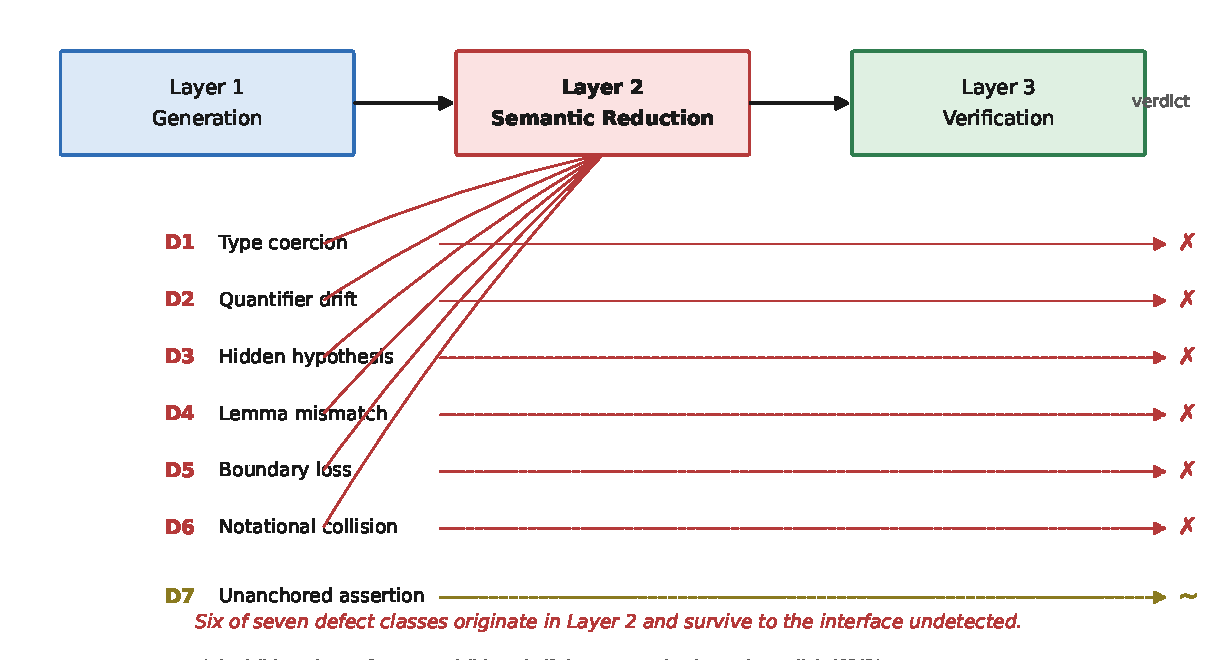
\includegraphics[width=0.78\textwidth]{fig2_defects.pdf}
\caption{Where the seven defect classes originate in the pipeline. Defects
D1--D6 arise in the mapping performed by Layer~2 and survive to the interface
undetected. D7 is partially visible because SRIR forces the assumption to be
represented explicitly rather than absorbed into prose.}
\label{fig:defects}
\end{figure}

% ============================================================================
\section{The Narrowing Hypothesis}
\label{sec:hypothesis}

We now state the central empirical claim of the framework. It is offered as a
falsifiable hypothesis, not a result.

\begin{quote}
\textbf{Narrowing hypothesis.} For an AI4Math system $\langle G, R, C\rangle$
and a benchmark $\mathcal{B}$, the rate of \emph{accepted-but-wrong} outputs is
bounded above by a function of the unanchored fraction $1 - \V$ of the
derivations the system accepts:
\[
  \Pr_{\substack{x \sim \mathcal{B} \\ C(G(x)) = \top}}\!\bigl[\,x \text{ is
  actually wrong}\,\bigr]
  \;\;\lesssim\;\;
  f\bigl(1 - \V(\mathcal{G}_x)\bigr)
\]
for some nondecreasing $f$ with $f(0) = 0$.
\end{quote}

The hypothesis says: \emph{a system whose accepted derivations are fully
anchored cannot be accepted-but-wrong, and as anchoring degrades, the rate of
accepted-but-wrong outputs rises}. The first half is essentially a restatement
of Proposition~\ref{prop:asymmetry} under the assumption that anchoring is
sound; the content is in the second half, which asserts a quantitative
relationship that could fail.

\subsection{Designing a test}

The hypothesis is testable with equipment that already exists. We sketch a
design and name its weaknesses, because a framework that cannot say how it would
be refuted is not doing useful work.

\begin{enumerate}
  \item \textbf{Construct derivations with controlled anchoring.} Take a set of
        problems with known formalisations. Generate derivations, then
        deliberately degrade them by injecting each defect class D1--D7 at a
        controlled rate, producing SRIR graphs with known $\V$.
  \item \textbf{Measure accepted-but-wrong rate.} For each derivation, run the
        verification layer and record acceptance. Where acceptance occurs,
        determine ground truth by comparing the formalised claim against the
        intended claim by human adjudication.
  \item \textbf{Fit and test.} Estimate $f$ and test whether the accepted-but-wrong
        rate is bounded by it. The hypothesis fails if the rate stays high at
        $\V \to 1$, or is insensitive to $1 - \V$.
\end{enumerate}

\subsection{Confounders and threats to validity}

We state these explicitly, in the spirit of the boundary conditions requested of
any framework claim.

\begin{itemize}
  \item \textbf{Adjudication cost.} Determining ``actually wrong'' requires
        comparing intended and formalised claims---the very anchoring gap we are
        studying. A cheap proxy is to use hand-formalised reference claims; this
        restricts the test to problems where a reference exists and biases
        toward well-formalised domains.
  \item \textbf{Degradation realism.} Injected defects may not resemble the
        defects a real model produces. A model's reduction errors are
        distributionally different from random injections, plausibly because
        they cluster in the directions the model finds convenient.
  \item \textbf{Weighting sensitivity.} $\V$ depends on the choice of $w$.
        Results should be reported under at least two weightings, e.g.\ the
        uniform and cone weightings, and the conclusion claimed only if they
        agree.
  \item \textbf{Closed-world bias.} Benchmarks drawn from well-formalised
        libraries have unusually reliable reduction because the informal and
        formal languages are close. Performance outside such domains is the
        case we are most interested in and the hardest to test.
\end{itemize}

\subsection{What the hypothesis is not}

It is not a claim that reducing unanchored steps is sufficient for reliability:
a fully anchored derivation of the wrong theorem is still the wrong theorem,
though the framing of ``wrong theorem'' is then resolved by the type system
rather than by a judgement call. Nor is it a claim that $\V$ is the only useful
measure; it is offered as a candidate axis that current benchmarks lack.

% ============================================================================
\section{A Reliability Checklist for AI4Math Claims}
\label{sec:checklist}

The framework's practical output is a checklist. It is designed for a
practitioner facing a claim of the form ``an AI system has established
mathematical result $X$'' and asking how much credence to extend. The full form
appears in Appendix~\ref{app:checklist}; we state the six questions here with
their rationale.

\begin{enumerate}
  \item \textbf{What exactly was formalised?} Obtain the formal statement, not
        only the informal gloss. If no formal statement exists, ask what the
        strongest available anchor is (a symbolic check, a numerical
        verification, an independent replication).
  \item \textbf{Is the informal-to-formal mapping disclosed step by step?} If
        the system reports only a final kernel verdict, the anchoring gap is
        undisclosed and D1--D6 are unauditable.
  \item \textbf{Which steps are anchored, and which are unanchored?} In SRIR
        terms, what is $\V$, and which nodes carry $\alpha = \mathsf{U}$?
  \item \textbf{Are the unanchored steps load-bearing?} A single unanchored
        step on the critical path matters more than several off it; this is what
        the cone weighting is for.
  \item \textbf{Do the library citations hold up?} Check that cited lemmas are
        applied within their stated hypotheses (D4), rather than matched by
        name.
  \item \textbf{What is the boundary of the claim?} Which domains, library
        coverage assumptions, and problem classes does the result depend on? A
        result established in a well-formalised closed domain does not transfer
        to an open one.
\end{enumerate}

The checklist is intentionally ordered by cost: questions 1--2 are answerable
from system outputs alone, questions 3--5 require instrumentation of the kind
SRIR provides, and question 6 is a judgement that no tool supplies.

% ============================================================================
\section{Discussion}
\label{sec:discussion}

\subsection{Implications for system design}

If the analysis is right, three design consequences follow.

First, \emph{the reduction layer deserves its own engineering effort and its own
evaluation}. Current systems invest in generation (better models) and
verification (better kernels and search) and treat reduction as glue. Our
analysis says the glue is load-bearing.

Second, \emph{disclosing the anchoring gap is more valuable than closing it}.
Closing it entirely is likely impossible for informal mathematics, which
depends on shared understanding that resists formalisation. Disclosing it is a
representation and interface problem, and our SRIR proposal is one concrete way
to do it.

Third, \emph{benchmarks should report verifiability alongside accuracy}. A
leaderboard that reports only final-answer correctness cannot distinguish a
system that reasoned soundly from one that got lucky, nor can it detect the
regression that occurs when a system becomes fluent faster than it becomes
sound.

\subsection{Limitations}
\label{sec:boundary}

We state plainly what this framework does not establish.

\begin{enumerate}
  \item \textbf{No empirical validation.} We present no experiments. The
        narrowing hypothesis is a proposal, and the taxonomy is a design
        artifact, not a validated instrument. Our citations to empirical work
        motivate the framework; they do not demonstrate it.
  \item \textbf{Annotation cost is unaddressed.} Producing SRIR graphs requires
        segmentation and per-step formalisation, both of which are themselves
        unreliable and potentially expensive. We have not measured this cost,
        and it may be prohibitive for long derivations.
  \item \textbf{The taxonomy is not exhaustive.} D1--D7 are drawn from the
        failure modes reported in the cited literature and our own analysis of
        worked examples. Other defect classes surely exist; we expect the list
        to be extended, and we regard it as a snapshot rather than a complete
        classification.
  \item \textbf{Semantic closure is strong.} Requiring every node in the cone of
        the root to be anchored is demanding, and may be unattainable for
        derivations that legitimately rely on standard results not yet in a
        library. The measure $\V$ exists partly to accommodate this, but the
        framework is likely most useful for well-formalised domains.
  \item \textbf{The framework assumes a formal target exists.} For mathematical
        activity that is not yet formalisable---conjecture generation,
        theory construction, taste and judgement---the analysis does not apply.
        These are exactly the activities that the creativity literature
        identifies as out of reach \cite{chen2025deepmath}.
\end{enumerate}

We consider limitation~5 the most important boundary. The framework addresses
\emph{reliability of claims already made}, not \emph{generation of good
claims}. A system with $\V = 1$ is trustworthy but not necessarily interesting.
Conflating the two would be the central error the framework is meant to prevent.

\subsection{Relation to the AGI-evaluation discourse}

The concern we formalise has a parallel in recent work on measuring general
capability. Assessment frameworks that decompose general intelligence into
distinct cognitive abilities---and that must therefore define what a given
measurement does and does not isolate---face the same attribution problem: a
score is only as meaningful as the construct it actually measures. The
reliability question we raise for AI4Math is the domain-specific version of this
general issue: \emph{what exactly is being certified, and does the certification
reach the claim that was made?} We regard this convergence as support for
treating construct validity as a first-class design concern rather than a
post-hoc statistical worry.

\subsection{Future work}

Three directions follow. (i)~Instrument an existing neuro-symbolic prover to
emit SRIR graphs and measure $\V$ on a standard benchmark, testing the narrowing
hypothesis. (ii)~Extend the taxonomy through systematic annotation of reduction
errors in a large corpus of model-generated formalisations, refining D1--D7 into
a validated instrument with inter-annotator agreement statistics. (iii)~Study
whether $\V$ can serve as a training signal, closing the loop between the
measurement and the reduction layer that the measure indicts.

% ============================================================================
\section{Conclusion}
\label{sec:conclusion}

Reliability in AI for Mathematics has been pursued as a verification problem:
add a checker, trust the checker. We have argued that this framing has a
structural blind spot. Because a proof assistant certifies the formal claim it
is given and is silent about whether that claim is the intended one, the
informal-to-formal reduction step can fail undetectably, and no improvement to
the checker addresses that failure. We located this blind spot at a specific
architectural position---the semantic reduction layer---and gave three
instruments for working with it: a typed intermediate representation that makes
anchoring explicit, a graded verifiability score that makes partial progress
measurable, and a defect taxonomy that gives failures names. We closed with a
falsifiable hypothesis and a checklist for practitioners.

The claim we would most like to see tested is the simplest one: that
disclosing which steps of a machine-produced proof are anchored, and which are
not, changes what we can responsibly conclude from it. If that is right, then
the next advance in reliable AI4Math will not be a stronger checker but a more
honest reduction layer.

% ============================================================================
\section*{Acknowledgements}

This work was conducted within the Elite~20 Program as a study of AI-assisted
academic research. The author thanks the authors of the reference materials for
making their lecture notes available. All large language model outputs used in
preparing this paper were independently verified against primary sources; the
verification record is maintained in the accompanying AI collaboration log.

% ============================================================================
\bibliographystyle{plain}
\bibliography{references}

% ============================================================================
\appendix

\section{Reliability Checklist (Full Form)}
\label{app:checklist}

The checklist below is intended to be applied in order. Each item states the
question, the evidence required, and the failure it detects.

\begin{table}[h]
\centering
\small
\caption{Full reliability checklist for auditing an AI4Math claim.}
\label{tab:checklist-full}
\begin{tabularx}{\textwidth}{@{}c l X l@{}}
\toprule
\textbf{\#} & \textbf{Question} & \textbf{Evidence required} & \textbf{Detects} \\
\midrule
1 & What was formalised? & Formal statement + informal source & --- \\
2 & Is the mapping disclosed? & Step-level correspondence & D1--D6 \\
3 & Which steps are anchored? & SRIR graph, $\alpha(\cdot)$ & D7 \\
4 & Are unanchored steps load-bearing? & Dependency cone & D7 \\
5 & Do library citations hold? & Lemma hypotheses vs.\ usage & D4 \\
6 & What is the claim's boundary? & Domain + coverage assumptions & D5 \\
7 & Does the result transfer? & Informal/formal language distance & D1, D6 \\
\bottomrule
\end{tabularx}
\end{table}

\section{A Worked SRIR Fragment}
\label{app:worked}

For concreteness we give the SRIR representation of a short derivation, showing
how anchoring status is recorded. The example is illustrative and uses a
schematic syntax rather than a specific implementation.

\begin{lstlisting}[caption={SRIR fragment for a two-step derivation. Note that the unanchored node is retained, not dropped, and that its status propagates to the goal.},label={lst:srir}]
( srir
  ( node n1 : type Assumption  : anchor U
      :gloss "n is a natural number greater than 1"
      :formal "n : Nat, h : n > 1"
      :note   "hypothesis stated informally but never
               discharged as an explicit premise" )

  ( node n2 : type LemmaRef    : anchor A
      :gloss "n has a prime factor by the fundamental theorem"
      :formal "Nat.exists_prime_and_dvd"
      :deps   (n1)
      :note   "lemma exists in mathlib; hypotheses match" )

  ( node n3 : type Goal        : anchor U
      :gloss "therefore n has a prime factor"
      :formal "exists p, Nat.Prime p AND p | n"
      :deps   (n2)
      :note   "status inherited from cone: n1 unanchored" ) )

; verifiability: V = 1/3 under uniform weighting
;                 semantic closure: FAILS at n1
; actionable:      promote the condition in n1 to an
;                  explicit premise; re-run anchoring pass
\end{lstlisting}

The fragment illustrates three properties of the representation. The unanchored
assertion is \emph{visible}: it appears as a node with $\alpha = \mathsf{U}$
rather than as a fluent sentence in a paragraph. The failure is
\emph{localised}: it is attributable to a specific node and a specific defect
class. And the remedy is \emph{stated}: the audit output says what would
change the verdict.

\end{document}
